\section{Abstraktní model křižovatky}\label{sec:krizovatka}

%Shrnutí hledání na grafu, definice grafu.
%
%Popis různých vzhledů křižovatky.
%Převod křižovatky na graf a parametry převodu.


Všechny mnou používané algoritmy jsou založeny na~prohledávání orientovaného grafu.
Z~tohoto důvodu je nutné převést křižovatku na~graf.
Převod je proveden rozdělením křižovatky na~diskrétní nepřekrývající~se bloky zaplňující celou plochu křižovatky.
Mezi sousedními bloky mohou auta přejíždět.

Formálně je křižovatka převedena na~orientovaný graf,
kde~každý blok je reprezentován jedním vrcholem a hrany vedou mezi bloky se společnou stěnou.
%Vzdálenost mezi sousedními bloky (čas přejezdu) je u~všech bloků stejný a trvá právě jeden krok simulace.  TODO

Bloky jsou rozděleny do~třech skupin.
První skupina jsou vrcholy reprezentující vnitřní plochu křižovatky.
Zbylé dvě skupiny reprezentují \hyperref[par:vjezdy]{vjezdy do~křižovatky} a \hyperref[par:vyjezdy]{výjezdy z~křižovatky}.

Rozhodl jsem se pro~$3$~různé typy křižovatek určené rozdělením plochy na~bloky.
Tyto~typy budu nazývat \hyperref[subsec:ctvercovy_typ]{čtvercový}, \hyperref[subsec:oktagonalni_typ]{oktagonální}
a~\hyperref[subsec:hexagonalni_typ]{hexagonální}.

Rozdělení křižovatky má určité parametry ovlivňující výsledný graf.
Těmito parametry jsou \hyperref[par:velikost_krizovatky]{velikost křižovatky},
\hyperref[par:vjezdy]{počet vjezdů} a~\hyperref[par:vyjezdy]{počet výjezdů}.

\paragraph{Velikost křižovatky}\label{par:velikost_krizovatky} značí z~kolika bloků se křižovatka skládá.
Obecně je hodnota \hyperref[par:velikost_krizovatky]{velikosti křižovatky} rovna počtu bloků na jedné hraně křižovatky.
Přesný význam je popsán zvlášť v~jednotlivých kapitolách.
Na~\hyperref[par:velikost_krizovatky]{velikosti křižovatky} závisí tzv.~\hyperref[par:velikost_bloku]{velikost bloku}.

\paragraph{Velikost bloku}\label{par:velikost_bloku} značí velikost základních bloků rozdělení
(odpovídá vzdálenosti mezi vrcholy), opět se ale u~různých typů liší.
Tuto~veličinu zavádím kvůli jednoduchému porovnání velikosti auta vůči bloku.

Každý typ křižovatky má předurčený počet \emph{směrů} ze~kterých auta přijíždějí.

\paragraph{Vjezdy}\label{par:vjezdy} značí množství vrcholů reprezentujících pruhy vjezdů z~každého \emph{směru} křižovatky.
Tyto vrcholy mají pouze jednu výstupní hranu a žádná hrana do nich nevede.

\paragraph{Výjezdy}\label{par:vyjezdy} mají podobný význam, určují počet výjezdních pruhů z~každého \emph{směru}.
Vrcholy výjezdů mají oproti \hyperref[par:vjezdy]{vjezdům} jednu vstupní hranu a žádnou výstupní.

Jelikož se na~silnicích auta pohybují po~pravé straně silnice,
jsou vjezdy a výjezdy z~jednoho směru seřazeny vůči hraně křižovatky zleva doprava v~pořadí
\ref{str:mezera_l}, \hyperref[par:vyjezdy]{výjezdy}, \ref{str:mezera_s}, \hyperref[par:vyjezdy]{vjezdy}, \ref{str:mezera_p}.
Kde~\emph{mezeraL}\labeltext{mezeraL}{str:mezera_l}, \emph{mezeraS}\labeltext{mezeraS}{str:mezera_s}
a~\emph{mezeraP}\labeltext{mezeraP}{str:mezera_p} značí posloupnost vrcholů na~hraně křižovatky
nesousedících s~vjezdem ani~výjezdem.
Všechny \hyperref[par:vjezdy]{vjezdy} jsou vždy přímo vedle sebe a \hyperref[par:vyjezdy]{výjezdy} taktéž.
Většina křižovatek je symetrická proto jsem určil, že velikost části \ref{str:mezera_l} bude shodná s~velikostí části \ref{str:mezera_p}.
Opět kvůli symetričnosti jsem zvolil velikost části \ref{str:mezera_p} co~nejblíže velikostem
krajových mezer \ref{str:mezera_l} a \ref{str:mezera_p}.
Platí tedy $\ref{str:mezera_l}=\ref{str:mezera_p}\wedge(\ref{str:mezera_s}=\ref{str:mezera_l}\vee\ref{str:mezera_s}+1=\ref{str:mezera_l})$.

\hyperref[par:pruh]{Pruhy} jsou známý koncept u křižovatek a v dopravě obecně.
Rozhodl jsem se proto formálně definovat \hyperref[par:pruh]{pruh}.

\paragraph{Pruh}\label{par:pruh} mezi určitým vjezdem a výjezdem definuji jako nejkratší cestu mezi těmito vrcholy.
Délka cesty je určena počtem vrcholů, přes které vede.
Pokud vedou dvě různé cesty přes stejný počet vrcholů, je upřednostněna ta, na~které musí auto méně zatáčet.
Čili cesty jsou následně porovnány podle úhlu, o~který se musí auta během jízdy otočit.
Pokud je i~tato hodnota stejná, porovnávají se auta podle počtu vrcholů, kterými neprojíždí rovně.
Při~posledním porovnání je preferována cesta s~více vrcholy.
Takto jsem se rozhodl, protože díky tomu budou mít auta méně ostré zatáčky.

\subsection{Čtvercový typ}\label{subsec:ctvercovy_typ}

\nameref{subsec:ctvercovy_typ} křižovatky rozděluje plochu do~čtvercových bloků.
Celková hlavní plocha křižovatky (tedy veškerá plocha mimo
\hyperref[par:vjezdy]{vjezdy} a \hyperref[par:vyjezdy]{výjezdy}) tvoří čtverec.

\nameref{par:velikost_krizovatky} značí počet bloků na~jedné straně plochy křižovatky.
Celkový počet bloků hlavní plochy křižovatky tudíž činí $g^2$,
kde $g$ je \hyperref[par:velikost_krizovatky]{velikost křižovatky}.
Pozice vrcholu je přesně uprostřed jemu odpovídajícího bloku.
Mezi každými bloky, který spolu sdílí stěnu, vede ve~výsledným grafu hrana.
Tento typ křižovatky má čtyři směry, jeden směr na~každé straně čtverce hlavní plochy.
Křižovatka je převedena na~graf s~$g^2 + 4i + 4o$ vrcholy,
kde $g$ opět značí \hyperref[par:velikost_krizovatky]{velikost},
$i$~\hyperref[par:vjezdy]{vjezdy} a $o$~\hyperref[par:vyjezdy]{výjezdy}.

Ukázka křižovatky s~\hyperref[par:velikost_krizovatky]{velikostí}~$4$, jedním \hyperref[par:vjezdy]{vjezdem} a
jedním \hyperref[par:vyjezdy]{výjezdem} je vidět na~obrázku~\ref{fig:square_type_graph}.
Na~obrázku jsou šedou barvou označeny vrcholy značící běžnou plochu křižovatky,
červeno-šedou barvou označeny vrcholy reprezentující \hyperref[par:vjezdy]{vjezdy} a
modro-šedé vrcholy reprezentují \hyperref[par:vyjezdy]{výjezdy}.

\begin{figure}[h]
	\centering
	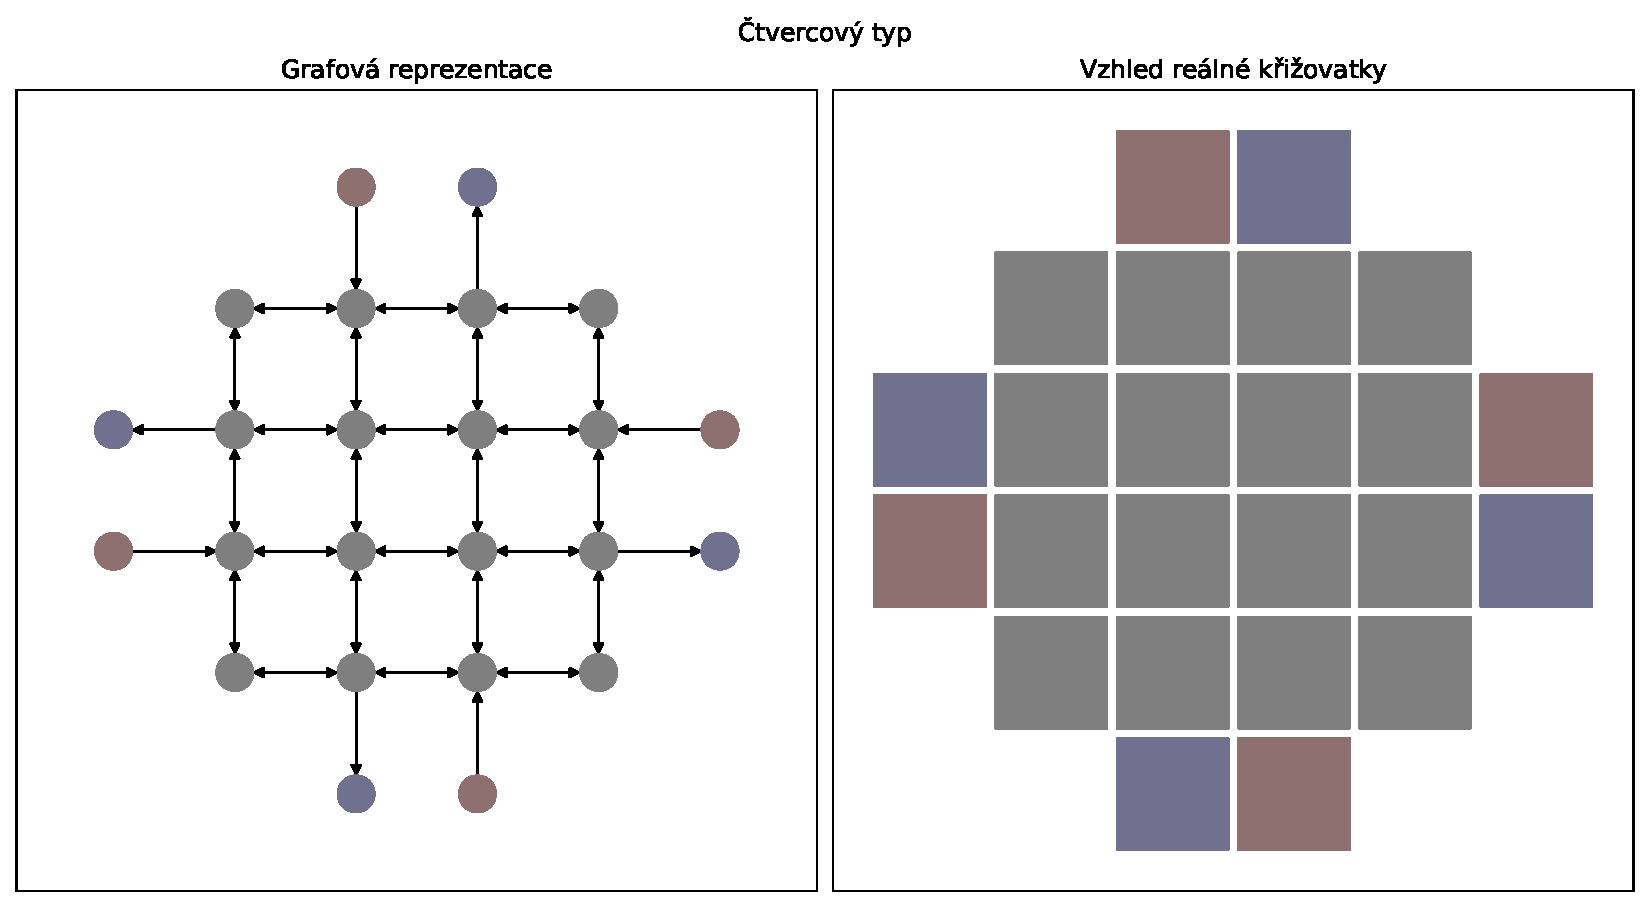
\includegraphics[width=\textwidth]{../img/Square_grid}
	\caption{Ukázka čtvercového typu křižovatky.}
	\label{fig:square_type_graph}
\end{figure}

\subsection{Oktagonální typ}\label{subsec:oktagonalni_typ}

\nameref{subsec:oktagonalni_typ} křižovatky vychází z~typu \hyperref[subsec:ctvercovy_typ]{čtvercového},
avšak rozšiřuje tento typ o~možnost diagonální jízdy.
Tohoto efektu docílí křižovatka přidáním dodatečných vrcholů mezi každé čtvercové bloky dotýkající se rohem.
Z~vizuálního hlediska se ze~čtvercových bloků stanou oktagonální (osmiúhelníkové),
odtud plyne samostatný název tohoto typu.
Tyto bloky mohou mít až~$8$~sousedů.
Mezi těmito oktagonálními bloky vzniknou nové bloky reprezentující diagonální přejezdy.
Nově vytvořené bloky mají nanejvýše $4$~sousedy, a tvoří pomyslný čtverec.
Z~vizuálních důvodů byly odebrány rohové bloky.

\nameref{par:velikost_krizovatky}, \hyperref[par:vjezdy]{vjezdy} a \hyperref[par:vyjezdy]{výjezdy}
mají stejný význam jako u~\hyperref[subsec:ctvercovy_typ]{čtvercového typu}.
Počet vrcholů u~této křižovatky činí $g^2 - 4 + (g-1)^2 + 4i + 4o = 2g^2 - 2g - 3 + 4(i + o)$,
kde $g$ je \hyperref[par:velikost_krizovatky]{velikost},
$i$ počet \hyperref[par:vjezdy]{vjezdů} a $o$ počet \hyperref[par:vyjezdy]{výjezdů}.
\nameref{par:velikost_bloku} je vzdálenost mezi dvěma sousedními vrcholy reprezentujícími oktagonální blok,
opět totožná s~velikostí bloku u~čtvercového typu.

Na~obrázku (Obrázek~\ref{fig:octagonal_type_graph}) je znázorněn příklad
\hyperref[subsec:oktagonali_typ]{oktagonálního typu} křižovatky s~\hyperref[par:velikost_krizovatky]{velikostí}~$4$,
jedním \hyperref[par:vjezdy]{vjezdem} a jedním \hyperref[par:vyjezdy]{výjezdem}.

Barvy vrcholů a bloků jsou stejné jako u~\hyperref[subsec:ctvercovy_typ]{čtvercového typu},
šedou barvou jsou označeny vrcholy značící běžnou plochu křižovatky,
červeno-šedou barvou označeny vrcholy reprezentující \hyperref[par:vjezdy]{vjezdy} a
modro-šedé vrcholy reprezentují \hyperref[par:vyjezdy]{výjezdy}.

\begin{figure}[h]
	\centering
	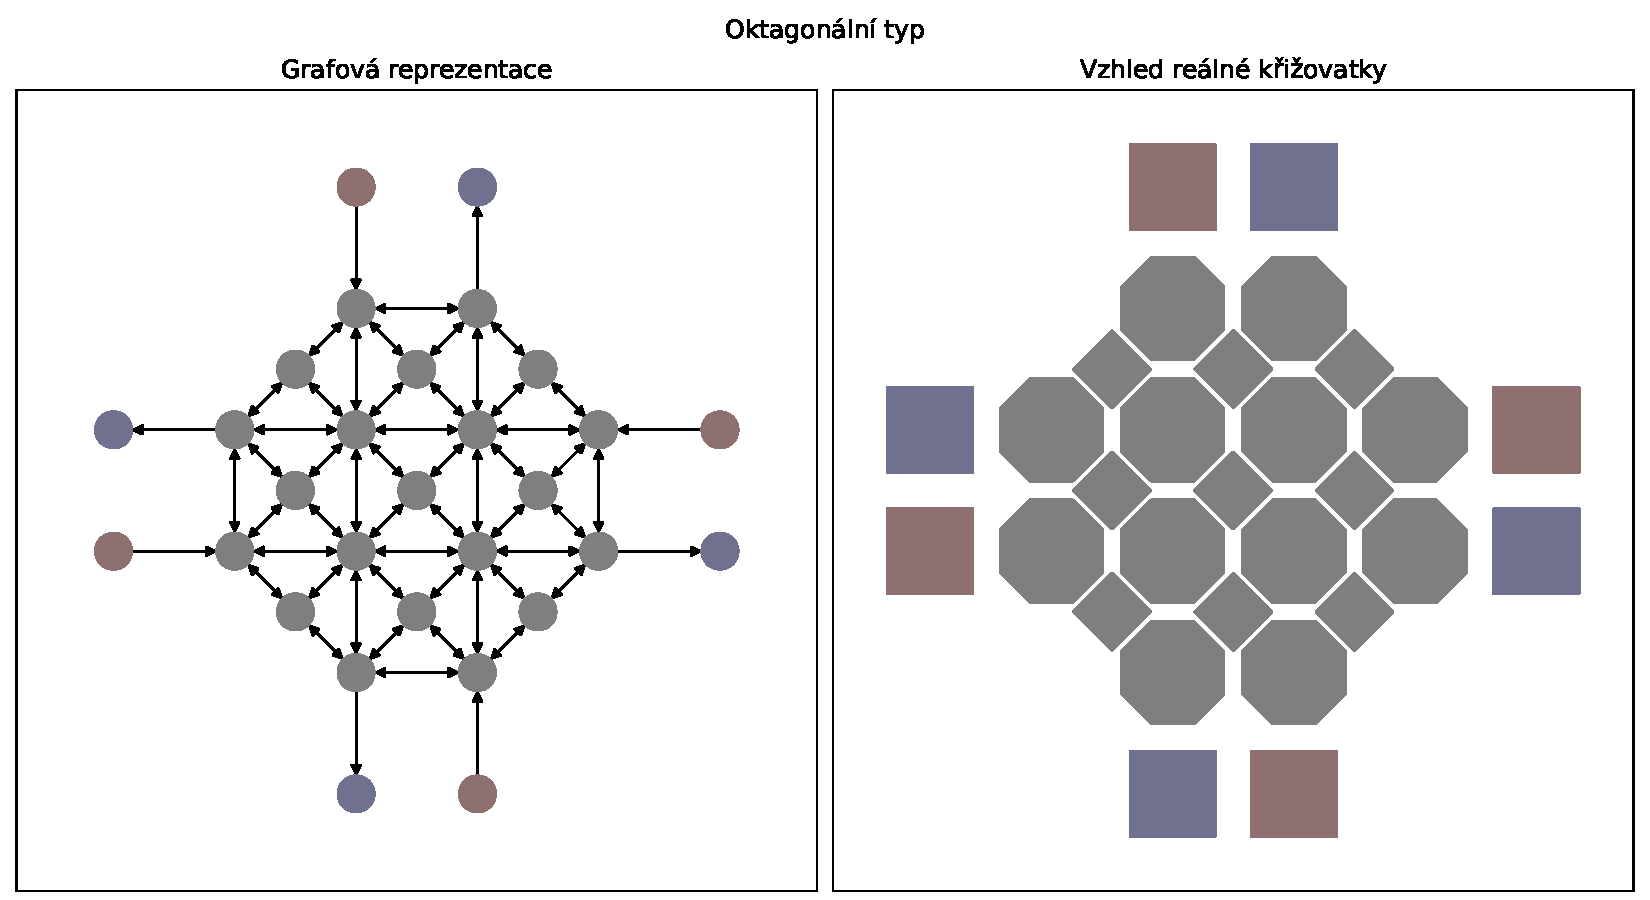
\includegraphics[width=\textwidth]{../img/Octagonal_grid}
	\caption{Ukázka oktagonálního typu křižovatky.}
	\label{fig:octagonal_type_graph}
\end{figure}

\subsection{Hexagonální typ}\label{subsec:hexagonalni_typ}

\nameref{subsec:hexagonalni_typ} je tvořen bloky s~tvary hexagonu (šestiúhelníku).
Při~převodu křižovatky na~graf je každý hexagonální blok nahrazen jedním vrcholem ležícím uprostřed původního bloku.
Opět hrany grafu vedou mezi bloky se společnou stěnou.
Každý blok má tedy až~$6$~sousedů.
Tyto bloky tvoří dohromady plochu tvaru velkého hexagonu.
Díky této reprezentaci má křižovatka tohoto typu $6$~směrů odkud mohou auta přijíždět.

Toto rozdělení sebou nese jednu velkou nevýhodu.
Pokud chce auto jet rovně skrze křižovatku (do~protilehlého směru), křižovatka mu nemůže nabídnout rovnou cestu.

\nameref{par:velikost_krizovatky} u~tohoto typu opět značí počet bloků na~jedné straně celkové plochy.
Hodnota je taktéž rovna počtu vrcholů z~kraje křižovatky do~středu.
Počet vrcholů grafu tedy činí $6 \times g \times (g-1) + 6i + 6o$,
kde $g$ je \hyperref[par:velikost_krizovatky]{velikost},
$i$ počet \hyperref[par:vjezdy]{vjezdů} a $o$ počet \hyperref[par:vyjezdy]{výjezdů}.
\nameref{par:velikost_bloku} je opět vzdálenost mezi dvěma sousedními vrcholy.

Na~obrázku (Obrázek~\ref{fig:hexagonal_type_graph}) je znázorněn příklad
\hyperref[subsec:hexagonalni_typ]{hexagonálního typu} křižovatky s~\hyperref[par:velikost_krizovatky]{velikostí}~$4$,
jedním \hyperref[par:vjezdy]{vjezdem} a jedním \hyperref[par:vyjezdy]{výjezdem}.

Barvy vrcholů a bloků jsou opět stejné.
Šedou barvou jsou označeny vrcholy značící běžnou plochu křižovatky,
červeno-šedou barvou označeny vrcholy reprezentující \hyperref[par:vjezdy]{vjezdy} a
modro-šedé vrcholy reprezentují \hyperref[par:vyjezdy]{výjezdy}.

\begin{figure}[h]
	\centering
	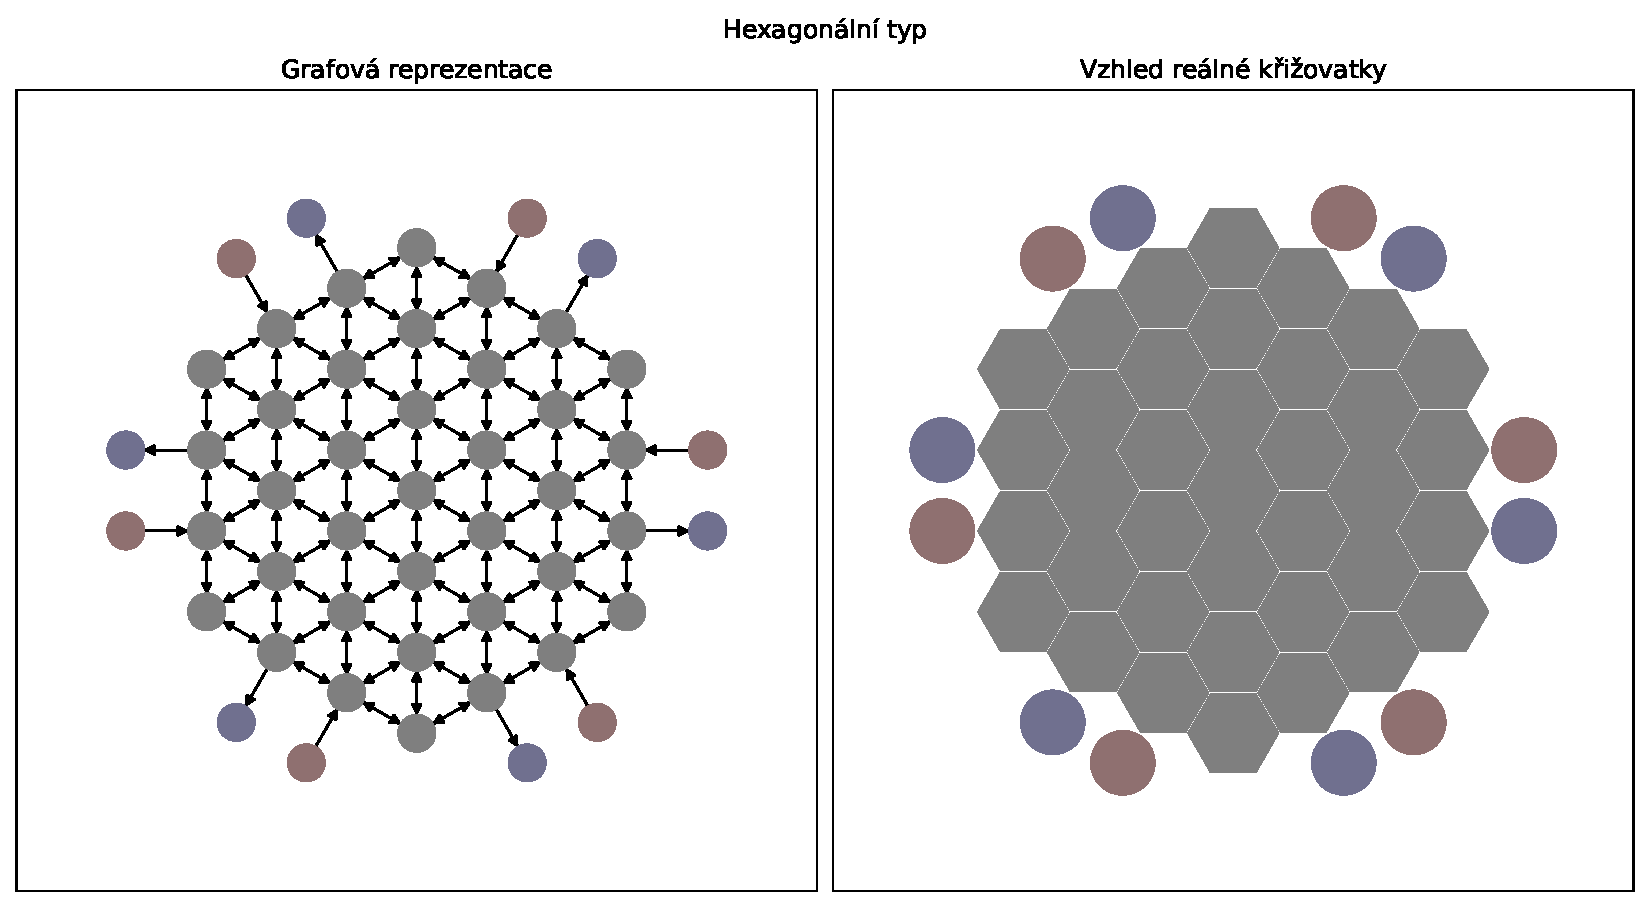
\includegraphics[width=\textwidth]{../img/Hexagonal_grid}
	\caption{Ukázka hexagonálního typu křižovatky.}
	\label{fig:hexagonal_type_graph}
\end{figure}
